% Options for packages loaded elsewhere
\PassOptionsToPackage{unicode}{hyperref}
\PassOptionsToPackage{hyphens}{url}
%
\documentclass[
]{article}
\usepackage{lmodern}
\usepackage{amssymb,amsmath}
\usepackage{ifxetex,ifluatex}
\ifnum 0\ifxetex 1\fi\ifluatex 1\fi=0 % if pdftex
  \usepackage[T1]{fontenc}
  \usepackage[utf8]{inputenc}
  \usepackage{textcomp} % provide euro and other symbols
\else % if luatex or xetex
  \usepackage{unicode-math}
  \defaultfontfeatures{Scale=MatchLowercase}
  \defaultfontfeatures[\rmfamily]{Ligatures=TeX,Scale=1}
\fi
% Use upquote if available, for straight quotes in verbatim environments
\IfFileExists{upquote.sty}{\usepackage{upquote}}{}
\IfFileExists{microtype.sty}{% use microtype if available
  \usepackage[]{microtype}
  \UseMicrotypeSet[protrusion]{basicmath} % disable protrusion for tt fonts
}{}
\makeatletter
\@ifundefined{KOMAClassName}{% if non-KOMA class
  \IfFileExists{parskip.sty}{%
    \usepackage{parskip}
  }{% else
    \setlength{\parindent}{0pt}
    \setlength{\parskip}{6pt plus 2pt minus 1pt}}
}{% if KOMA class
  \KOMAoptions{parskip=half}}
\makeatother
\usepackage{xcolor}
\IfFileExists{xurl.sty}{\usepackage{xurl}}{} % add URL line breaks if available
\IfFileExists{bookmark.sty}{\usepackage{bookmark}}{\usepackage{hyperref}}
\hypersetup{
  pdftitle={Comparative methods for measuring memory weight},
  pdfauthor={ROBINE Thomas},
  hidelinks,
  pdfcreator={LaTeX via pandoc}}
\urlstyle{same} % disable monospaced font for URLs
\usepackage[margin=1in]{geometry}
\usepackage{color}
\usepackage{fancyvrb}
\newcommand{\VerbBar}{|}
\newcommand{\VERB}{\Verb[commandchars=\\\{\}]}
\DefineVerbatimEnvironment{Highlighting}{Verbatim}{commandchars=\\\{\}}
% Add ',fontsize=\small' for more characters per line
\usepackage{framed}
\definecolor{shadecolor}{RGB}{248,248,248}
\newenvironment{Shaded}{\begin{snugshade}}{\end{snugshade}}
\newcommand{\AlertTok}[1]{\textcolor[rgb]{0.94,0.16,0.16}{#1}}
\newcommand{\AnnotationTok}[1]{\textcolor[rgb]{0.56,0.35,0.01}{\textbf{\textit{#1}}}}
\newcommand{\AttributeTok}[1]{\textcolor[rgb]{0.77,0.63,0.00}{#1}}
\newcommand{\BaseNTok}[1]{\textcolor[rgb]{0.00,0.00,0.81}{#1}}
\newcommand{\BuiltInTok}[1]{#1}
\newcommand{\CharTok}[1]{\textcolor[rgb]{0.31,0.60,0.02}{#1}}
\newcommand{\CommentTok}[1]{\textcolor[rgb]{0.56,0.35,0.01}{\textit{#1}}}
\newcommand{\CommentVarTok}[1]{\textcolor[rgb]{0.56,0.35,0.01}{\textbf{\textit{#1}}}}
\newcommand{\ConstantTok}[1]{\textcolor[rgb]{0.00,0.00,0.00}{#1}}
\newcommand{\ControlFlowTok}[1]{\textcolor[rgb]{0.13,0.29,0.53}{\textbf{#1}}}
\newcommand{\DataTypeTok}[1]{\textcolor[rgb]{0.13,0.29,0.53}{#1}}
\newcommand{\DecValTok}[1]{\textcolor[rgb]{0.00,0.00,0.81}{#1}}
\newcommand{\DocumentationTok}[1]{\textcolor[rgb]{0.56,0.35,0.01}{\textbf{\textit{#1}}}}
\newcommand{\ErrorTok}[1]{\textcolor[rgb]{0.64,0.00,0.00}{\textbf{#1}}}
\newcommand{\ExtensionTok}[1]{#1}
\newcommand{\FloatTok}[1]{\textcolor[rgb]{0.00,0.00,0.81}{#1}}
\newcommand{\FunctionTok}[1]{\textcolor[rgb]{0.00,0.00,0.00}{#1}}
\newcommand{\ImportTok}[1]{#1}
\newcommand{\InformationTok}[1]{\textcolor[rgb]{0.56,0.35,0.01}{\textbf{\textit{#1}}}}
\newcommand{\KeywordTok}[1]{\textcolor[rgb]{0.13,0.29,0.53}{\textbf{#1}}}
\newcommand{\NormalTok}[1]{#1}
\newcommand{\OperatorTok}[1]{\textcolor[rgb]{0.81,0.36,0.00}{\textbf{#1}}}
\newcommand{\OtherTok}[1]{\textcolor[rgb]{0.56,0.35,0.01}{#1}}
\newcommand{\PreprocessorTok}[1]{\textcolor[rgb]{0.56,0.35,0.01}{\textit{#1}}}
\newcommand{\RegionMarkerTok}[1]{#1}
\newcommand{\SpecialCharTok}[1]{\textcolor[rgb]{0.00,0.00,0.00}{#1}}
\newcommand{\SpecialStringTok}[1]{\textcolor[rgb]{0.31,0.60,0.02}{#1}}
\newcommand{\StringTok}[1]{\textcolor[rgb]{0.31,0.60,0.02}{#1}}
\newcommand{\VariableTok}[1]{\textcolor[rgb]{0.00,0.00,0.00}{#1}}
\newcommand{\VerbatimStringTok}[1]{\textcolor[rgb]{0.31,0.60,0.02}{#1}}
\newcommand{\WarningTok}[1]{\textcolor[rgb]{0.56,0.35,0.01}{\textbf{\textit{#1}}}}
\usepackage{graphicx,grffile}
\makeatletter
\def\maxwidth{\ifdim\Gin@nat@width>\linewidth\linewidth\else\Gin@nat@width\fi}
\def\maxheight{\ifdim\Gin@nat@height>\textheight\textheight\else\Gin@nat@height\fi}
\makeatother
% Scale images if necessary, so that they will not overflow the page
% margins by default, and it is still possible to overwrite the defaults
% using explicit options in \includegraphics[width, height, ...]{}
\setkeys{Gin}{width=\maxwidth,height=\maxheight,keepaspectratio}
% Set default figure placement to htbp
\makeatletter
\def\fps@figure{htbp}
\makeatother
\setlength{\emergencystretch}{3em} % prevent overfull lines
\providecommand{\tightlist}{%
  \setlength{\itemsep}{0pt}\setlength{\parskip}{0pt}}
\setcounter{secnumdepth}{-\maxdimen} % remove section numbering

\title{Comparative methods for measuring memory weight}
\author{ROBINE Thomas}
\date{20 février 2020}

\begin{document}
\maketitle

\hypertarget{introduction}{%
\section{Introduction}\label{introduction}}

We want to know the best way to determine the memory weight of a
datatype structure, especially for the ``Reference Class'' type, which
is quite difficult to evaluate. Currently, we're using the object.size()
method in order to calculate the memory weight of the datatype structure
in the ``data\_structure\_creations\_tests.Rmd'' document and we're
searching for a new and more efficient method. For that we have 3
differents ways to measure it (object.size() from utils package,
obj\_size() from lobstr package and memuse from itself package).

\begin{Shaded}
\begin{Highlighting}[]
\KeywordTok{source}\NormalTok{(}\StringTok{"data_structure_functions.R"}\NormalTok{)}
\KeywordTok{library}\NormalTok{(tibble)}
\KeywordTok{library}\NormalTok{(data.table)}
\KeywordTok{library}\NormalTok{(tidyverse)}
\end{Highlighting}
\end{Shaded}

\begin{verbatim}
## -- Attaching packages -------------------------------------------------------------------------------- tidyverse 1.3.0 --
\end{verbatim}

\begin{verbatim}
## v ggplot2 3.3.0     v dplyr   0.8.5
## v tidyr   1.0.2     v stringr 1.4.0
## v readr   1.3.1     v forcats 0.5.0
## v purrr   0.3.3
\end{verbatim}

\begin{verbatim}
## -- Conflicts ----------------------------------------------------------------------------------- tidyverse_conflicts() --
## x dplyr::between()   masks data.table::between()
## x dplyr::filter()    masks stats::filter()
## x dplyr::first()     masks data.table::first()
## x dplyr::lag()       masks stats::lag()
## x dplyr::last()      masks data.table::last()
## x purrr::transpose() masks data.table::transpose()
\end{verbatim}

\begin{Shaded}
\begin{Highlighting}[]
\KeywordTok{library}\NormalTok{(microbenchmark)}
\KeywordTok{library}\NormalTok{(dplyr)}
\KeywordTok{library}\NormalTok{(ggplot2)}
\KeywordTok{library}\NormalTok{(memuse)}
\KeywordTok{library}\NormalTok{(lobstr)}
\KeywordTok{options}\NormalTok{(}\DataTypeTok{warn=}\OperatorTok{-}\DecValTok{1}\NormalTok{)}

\NormalTok{size <-}\StringTok{ }\KeywordTok{c}\NormalTok{(}\DecValTok{10000}\NormalTok{,}\DecValTok{100000}\NormalTok{)}\CommentTok{#,1000000)}

\ControlFlowTok{for}\NormalTok{ (i }\ControlFlowTok{in}\NormalTok{ size) \{}
\NormalTok{  liste <-}\StringTok{ }\KeywordTok{list_of_usm_list_by_vector}\NormalTok{(i)}
\NormalTok{  classe <-}\StringTok{ }\KeywordTok{list_of_usm_list_by_vector}\NormalTok{(i)}
\NormalTok{  df <-}\StringTok{ }\KeywordTok{usm_dataframe_by_vector}\NormalTok{(i)}
\NormalTok{  dt <-}\StringTok{ }\KeywordTok{usm_datatable_by_usm_dataframe_by_vector}\NormalTok{(i)}
\NormalTok{  tb <-}\StringTok{ }\KeywordTok{usm_tibble_by_usm_dataframe_by_vector}\NormalTok{(i)}
  
\NormalTok{  all_weight <-}\StringTok{ }\KeywordTok{object.size}\NormalTok{(liste)}
\NormalTok{  all_weight <-}\StringTok{ }\KeywordTok{append}\NormalTok{(all_weight,}\KeywordTok{object.size}\NormalTok{(classe))}
\NormalTok{  all_weight <-}\StringTok{ }\KeywordTok{append}\NormalTok{(all_weight,}\KeywordTok{object.size}\NormalTok{(df))}
\NormalTok{  all_weight <-}\StringTok{ }\KeywordTok{append}\NormalTok{(all_weight,}\KeywordTok{object.size}\NormalTok{(dt))}
\NormalTok{  all_weight <-}\StringTok{ }\KeywordTok{append}\NormalTok{(all_weight,}\KeywordTok{object.size}\NormalTok{(tb))}
  
\NormalTok{  all_weight <-}\StringTok{ }\KeywordTok{append}\NormalTok{(all_weight,}\KeywordTok{obj_size}\NormalTok{(liste))}
\NormalTok{  all_weight <-}\StringTok{ }\KeywordTok{append}\NormalTok{(all_weight,}\KeywordTok{obj_size}\NormalTok{(classe))}
\NormalTok{  all_weight <-}\StringTok{ }\KeywordTok{append}\NormalTok{(all_weight,}\KeywordTok{obj_size}\NormalTok{(df))}
\NormalTok{  all_weight <-}\StringTok{ }\KeywordTok{append}\NormalTok{(all_weight,}\KeywordTok{obj_size}\NormalTok{(dt))}
\NormalTok{  all_weight <-}\StringTok{ }\KeywordTok{append}\NormalTok{(all_weight,}\KeywordTok{obj_size}\NormalTok{(tb))}
  
\NormalTok{  all_weight <-}\StringTok{ }\KeywordTok{append}\NormalTok{(all_weight,}\KeywordTok{as.numeric}\NormalTok{(}\KeywordTok{memuse}\NormalTok{(liste)))}
\NormalTok{  all_weight <-}\StringTok{ }\KeywordTok{append}\NormalTok{(all_weight,}\KeywordTok{as.numeric}\NormalTok{(}\KeywordTok{memuse}\NormalTok{(classe)))}
\NormalTok{  all_weight <-}\StringTok{ }\KeywordTok{append}\NormalTok{(all_weight,}\KeywordTok{as.numeric}\NormalTok{(}\KeywordTok{memuse}\NormalTok{(df)))}
\NormalTok{  all_weight <-}\StringTok{ }\KeywordTok{append}\NormalTok{(all_weight,}\KeywordTok{as.numeric}\NormalTok{(}\KeywordTok{memuse}\NormalTok{(dt)))}
\NormalTok{  all_weight <-}\StringTok{ }\KeywordTok{append}\NormalTok{(all_weight,}\KeywordTok{as.numeric}\NormalTok{(}\KeywordTok{memuse}\NormalTok{(tb)))}
  
\NormalTok{  Structures_types <-}\StringTok{ }\KeywordTok{c}\NormalTok{(}\StringTok{"List"}\NormalTok{,}\StringTok{"Class"}\NormalTok{,}\StringTok{"Dataframe"}\NormalTok{,}\StringTok{"Datatable"}\NormalTok{,}\StringTok{"Tibble"}\NormalTok{)}
\NormalTok{  structures <-}\StringTok{ }\KeywordTok{rep}\NormalTok{(Structures_types,}\DecValTok{3}\NormalTok{)}
\NormalTok{  weight_log10 <-}\StringTok{ }\KeywordTok{log10}\NormalTok{(all_weight)}
\NormalTok{  methods <-}\StringTok{ }\KeywordTok{c}\NormalTok{(}\KeywordTok{rep}\NormalTok{(}\StringTok{"object.size"}\NormalTok{,}\DecValTok{5}\NormalTok{),}\KeywordTok{rep}\NormalTok{(}\StringTok{"obj_size"}\NormalTok{,}\DecValTok{5}\NormalTok{),}\KeywordTok{rep}\NormalTok{(}\StringTok{"memuse"}\NormalTok{,}\DecValTok{5}\NormalTok{))}
  
\NormalTok{  global_plot_weight_recap <-}\StringTok{ }\KeywordTok{data.frame}\NormalTok{(structures,weight_log10,methods)}
  
\NormalTok{  global_graph_weight_recap <-}\StringTok{ }\KeywordTok{ggplot}\NormalTok{(}\DataTypeTok{data =}\NormalTok{ global_plot_weight_recap,}\KeywordTok{aes}\NormalTok{(}\DataTypeTok{x =}\NormalTok{ methods, }\DataTypeTok{y=}\NormalTok{weight_log10, }\DataTypeTok{fill =}\NormalTok{ structures)) }\OperatorTok{+}
\StringTok{    }\KeywordTok{geom_bar}\NormalTok{(}\DataTypeTok{position =} \StringTok{"dodge"}\NormalTok{, }\DataTypeTok{stat =} \StringTok{"identity"}\NormalTok{)}
  \KeywordTok{print}\NormalTok{(global_graph_weight_recap }\OperatorTok{+}\StringTok{ }\KeywordTok{ggtitle}\NormalTok{(}\KeywordTok{sprintf}\NormalTok{(}\StringTok{"%s %d"}\NormalTok{,}\StringTok{"weight measure method recap graph for size ="}\NormalTok{,i)))}
\NormalTok{\}}
\end{Highlighting}
\end{Shaded}

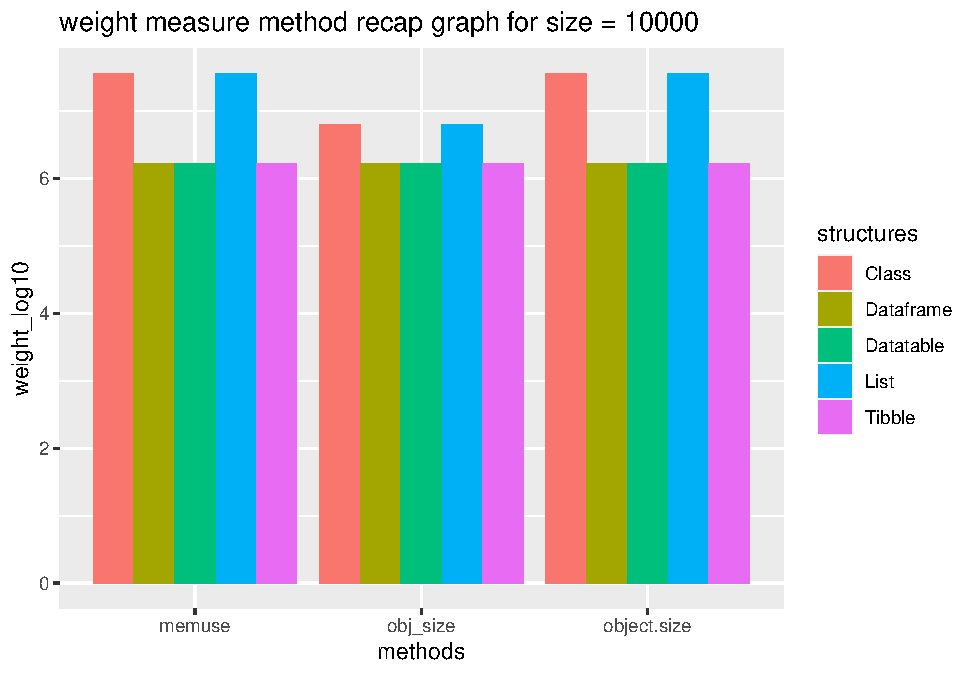
\includegraphics{comparative_methods_for_measuring_memory_weight_files/figure-latex/code-1.pdf}
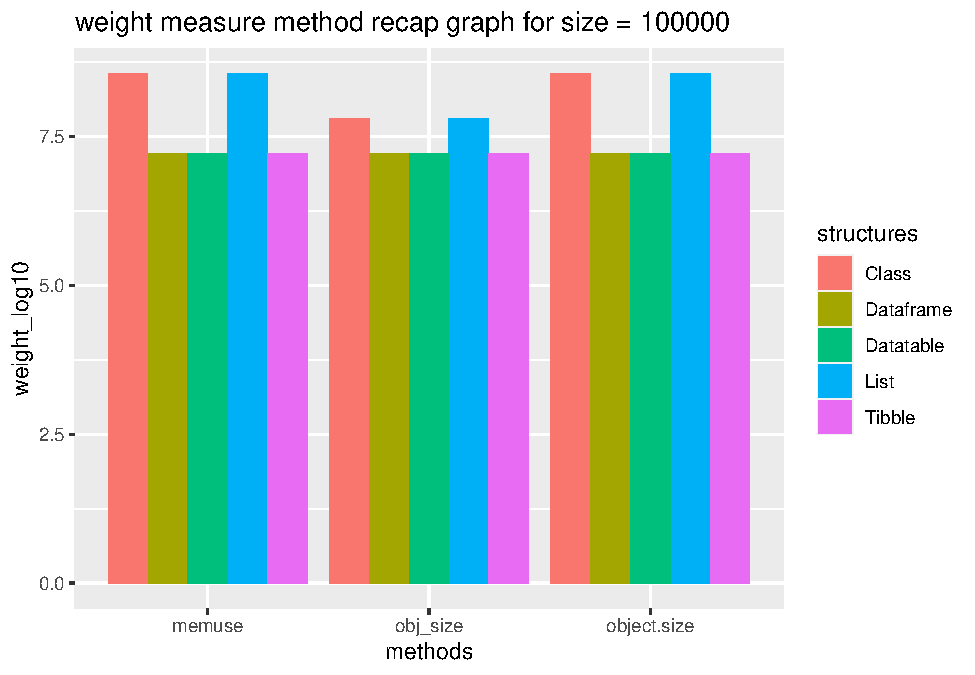
\includegraphics{comparative_methods_for_measuring_memory_weight_files/figure-latex/code-2.pdf}

\hypertarget{conclusion}{%
\section{Conclusion}\label{conclusion}}

Firstly, the ``Reference Class'' type was the datatype structure with
the lower memory weight, but due to some modifications in the generation
functions in ``data\_structure\_functions.R'', it is not the case
anymore. To conclude, we can still continue to use object.size().

\end{document}
